\chapter{Results}

The data from a total of 23 participants with the average of 335 and a total of 7708 trials were used for the analysis. The starting location IDs were identical with the building-IDs inside the unity environment and were not replaced with new numbers for the analysis.

\section{Summary statistics of dependent variables}

\subsection{Absolute angular deviation}

This variable has the mean of 48.08 with the standard deviation of 44.30, and median of 33.70. (See figure \ref{fig:angular_dev_dists})

\begin{figure}[!htb]
	\centering
	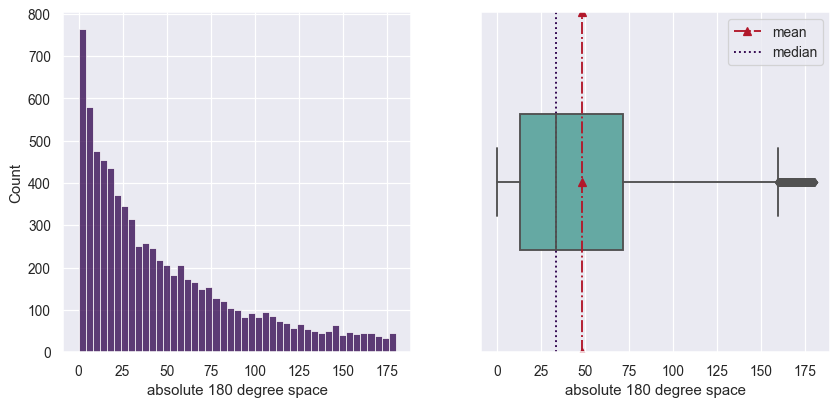
\includegraphics[width=150mm]{figures/angular_deviation_hist_box_23.png}
	\caption[Distribution of the absolute angular deviation]{distribution of the absolute angular deviation}
	\label{fig:angular_dev_dists}
\end{figure}

\subsection{Reaction times}

This variable has the mean of 7.77 with the standard deviation of 5.56, and median of 6.06. (See figure \ref{fig:rt_dists})

\begin{figure}[!htb]
	\centering
	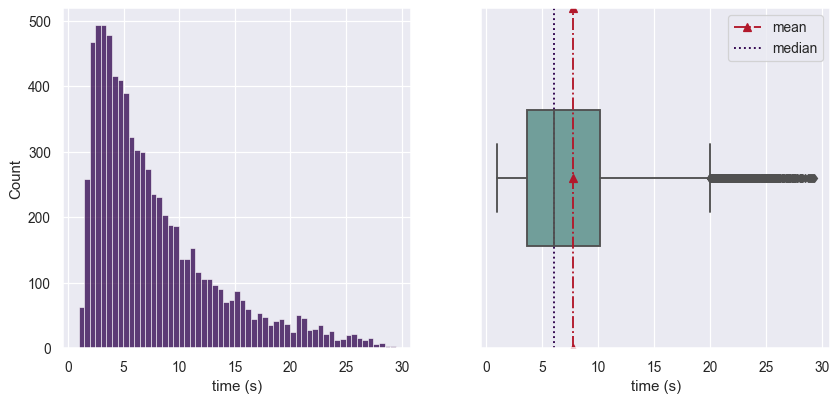
\includegraphics[width=150mm]{figures/RT_hist_box_23.png}
	\caption[Distribution of reaction times]{distribution of the  reaction times in the pointing task}
	\label{fig:rt_dists}
\end{figure}

\section{Extremes at starting locations}

\subsection{Absolute angular deviation}

In order to find out which of the 28 starting locations were the best and worst in performance with respect to the angular deviation from the target, the minimum and maximum medians of angular deviation grouped by the starting locations were taken.\\
As a result the starting location with the ID 9 which is a patisserie shop, therefore a context meaningful location, with the median of 19.18 degree deviation from the targets and the difference of 16.03 degree from the overall median (35.21) is the best location, i.e., has the lowest degree deviation from the target. See figure \ref{fig:best_angular}.\\

\begin{figure}[!htb]
	\centering
	\begin{subfigure}[b]{0.48\linewidth}
		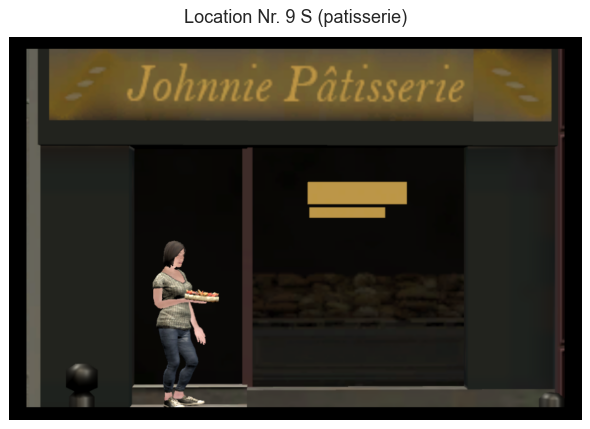
\includegraphics[width=\linewidth]{figures/best_loc_angular_error_withHA_23.png}
		\caption{best starting location}
		\label{fig:best_angular}
	\end{subfigure}
	\begin{subfigure}[b]{0.48\linewidth}
		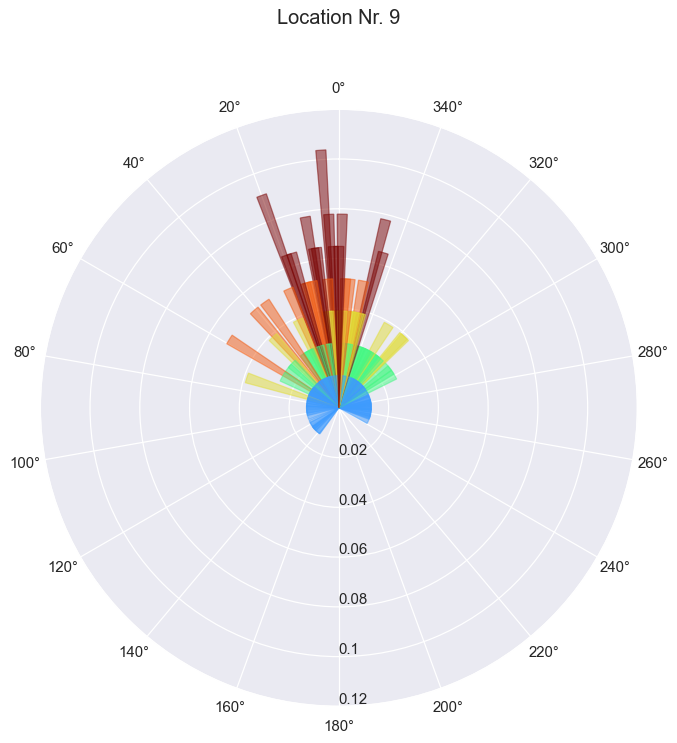
\includegraphics[width=\linewidth]{figures/deviation_degrees_loc_nr_9_23.png}
		\caption{angular deviation at location 9 (\%)}
		\label{fig:best_angular_dist_9}
	\end{subfigure}
	
	\caption[Best starting location based on angular deviation]{the best starting location is chosen by taking the least median angular deviation among all starting locations.}
\end{figure}
\label{fig:best_location}

Furthermore, the starting location with the ID 35, one of the residential, thus not context meaningful buildings, with the angular deviation median of 52.49 degree away from the target and overall distance of 17.28 degree from the overall median (35.21) was the worst location of performing the task with regard to the angular deviation. See figure \ref{fig:worst_angular}.

\begin{figure}[!htb]
	\begin{subfigure}[b]{0.48\linewidth}
		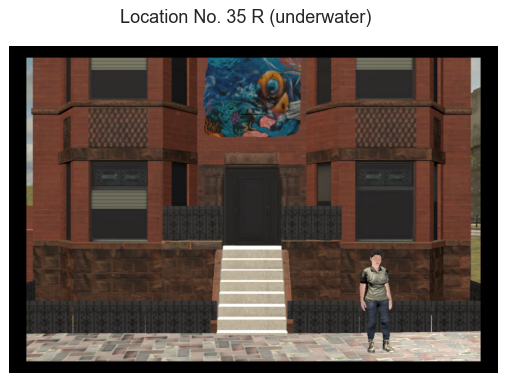
\includegraphics[width=\linewidth]{figures/worst_loc_angular_error__withHA_23.png}
		\caption{worst starting location}
		\label{fig:worst_angular}
	\end{subfigure}
	\begin{subfigure}[b]{0.48\linewidth}
		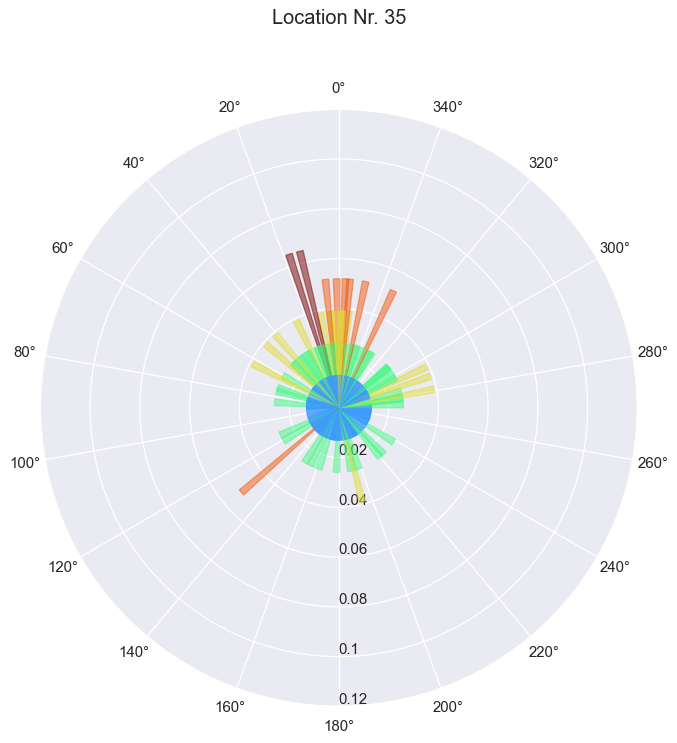
\includegraphics[width=\linewidth]{figures/deviation_degrees_loc_nr_35_23.png}
		\caption{angular deviation at location 35 (\%)}
		\label{fig:worst_angular_dist_35}
	\end{subfigure}

	\caption[Worst starting location based on angular deviation]{the worst starting location is chosen by taking the highest median angular deviation among all starting locations.}
\end{figure}
\label{fig:worst_location}

\begin{figure}[!htb]
	\centering
	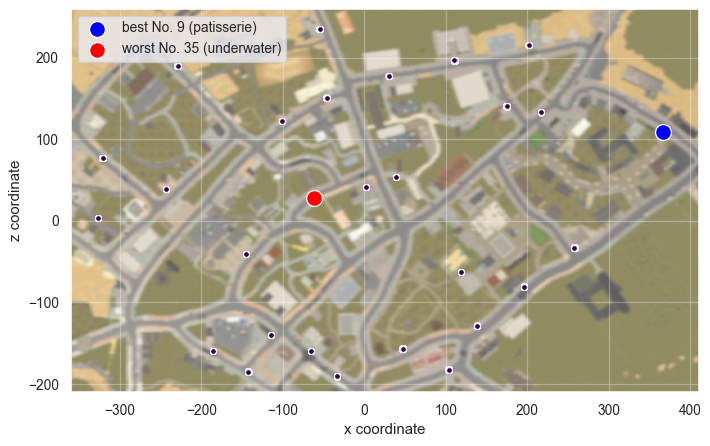
\includegraphics[width=140mm]{figures/best_worst_starting_locations_map.png}
	\caption[Locations of best and worst starting locations in city]{the locations of the best and worst starting locations inside the city coordinates.}
	\label{fig:best_worst_locs}
\end{figure}


\subsection{Reaction times}

For finding the fastest and the slowest performance among the 28 starting locations, the medians of reaction times grouped by the starting locations were Calculated.\\
The starting location number 51 which was a wine shop, hence a context meaningful location, with the median of 4.63s and the difference of 1.38s from the overall median (6.01) was the fastest location. See figure \ref{fig:fastest_loc}.\\

\begin{figure}[!htb]
	\centering
	\begin{subfigure}[b]{0.48\linewidth}
		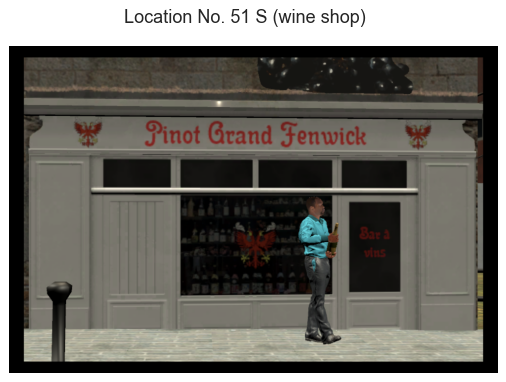
\includegraphics[width=\linewidth]{figures/fastest_loc_RT_withHA_23.png}
		\caption{fastest starting location}
		\label{fig:fastest_loc}
	\end{subfigure}
	\begin{subfigure}[b]{0.48\linewidth}
		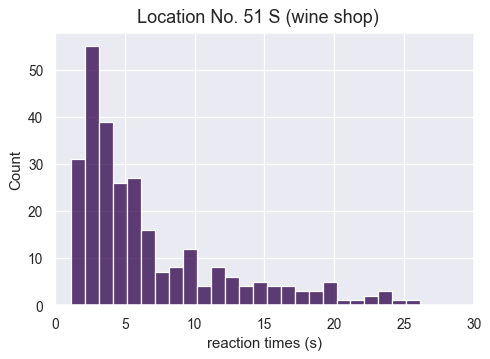
\includegraphics[width=\linewidth]{figures/fastest_loc_RT_dist_51_23.png}
		\caption{reaction times at location 51 (\%)}
		\label{fig:fastest_loc_dist}
	\end{subfigure}
	
	\caption[Fastest starting location]{the fastest starting location is chosen by taking the least median reaction time among all starting locations.}
\end{figure}
\label{fig:fastest_location}


Furthermore, the starting location 35, the residential not context meaningful location with the worst angular deviation performance with the median of 7.75s and overall distance of 1.74s from the overall median (6.01) was the slowest location among the 28. See figure \ref{fig:slowest_loc}.

\begin{figure}[!htb]
	\begin{subfigure}[b]{0.48\linewidth}
		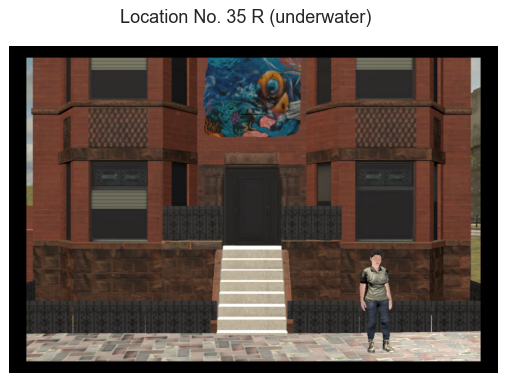
\includegraphics[width=\linewidth]{figures/worst_loc_angular_error__withHA_23.png}
		\caption{slowest starting location}
		\label{fig:slowest_loc}
	\end{subfigure}
	\begin{subfigure}[b]{0.48\linewidth}
		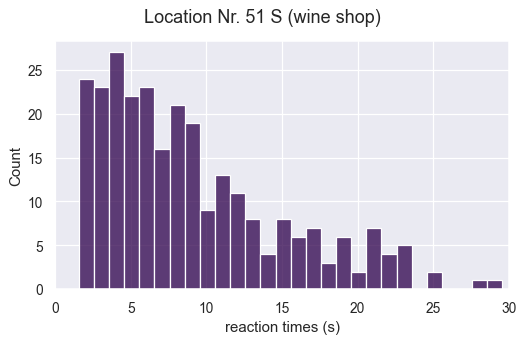
\includegraphics[width=\linewidth]{figures/slowest_loc_RT_dist_35_23.png}
		\caption{distribution of reaction times at location 35 (\%)}
		\label{fig:best_angular_dist_35}
	\end{subfigure}
	
	\caption[Slowest starting location]{the slowest starting location is chosen by taking the highest median of reaction times among all starting locations.}
\end{figure}
\label{fig:slowest_location}

\begin{figure}[!htb]
	\centering
	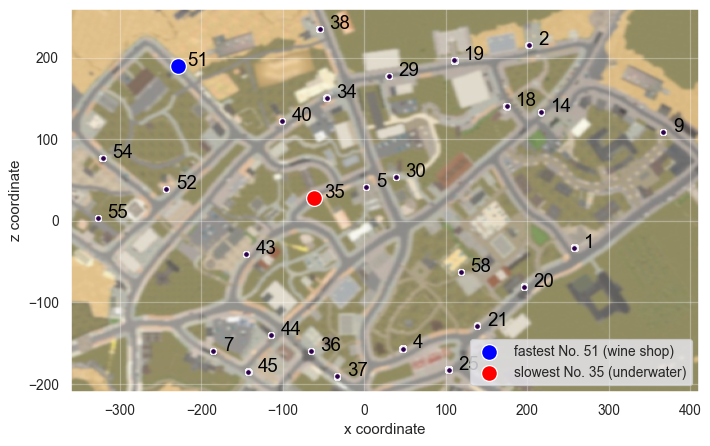
\includegraphics[width=140mm]{figures/fastest_slowest_starting_locations_RT_map.png}
	\caption[Locations of fastest and slowest starting locations in city]{the locations of the fastest and the slowest starting locations inside the city coordinates.}
	\label{fig:fastest_slowest_locs}
\end{figure}

\section{Linear mixed effects model}

\subsection{Absolute angular deviation}

For choosing the intercept for the model the overall mean of absolute angular deviation, 48.09 degree, was taken into account. The starting location No. 20 (fast food) which is a meaningful location with the mean absolute angular deviation 48.07 was chosen since its mean absolute angular deviation was the closest to the overall mean among starting locations by 0.02 degree absolute difference.

The LMM model was fitted using that reference location No. 20. The results (see table \ref{tab:angle_loc}) show a significant effect of 12 starting locations listed in the table \ref{tab:sig_angle_loc} on the dependent variable. From the 12 locations with a significant effect, 7 are meaningful locations and from the 15 non-significant locations, 6 are meaningful (see figure \ref{fig:sig_angle_loc_map}). The variance between subjects is 174.867. 
                                                                                            
                                                                                   \rowcolors{1}{light-gray}{light-gray}
\begin{longtable}{p{4cm}p{2cm}p{2cm}p{2cm}l}
	\hiderowcolors
	\caption[Absolute angular deviation by starting locations]{The results of the model absolute angular deviation by starting locations. "Loc" stands for location. z-score(=$\beta/SE(\beta)$)} \\ [5ex]
	

	\hline \hline 
	\multicolumn{1}{l}{Predictor} & \multicolumn{1}{l}{Coef. $\beta$} & \multicolumn{1}{l}{SE ($\beta$)} & \multicolumn{1}{l}{z-score} & \multicolumn{1}{r}{P$>|z|$} \\
	\hline \hline
	\showrowcolors
	Intercept    & 48.066  & 3.717 & 12.933 & \textbf{\boldmath{\textless}.001} \\
	{[}Loc.1{]}  & -1.335  & 3.524 & -0.379 & 0.705 \\
	\setrow{\bfseries} {[}Loc.2{]}  & \setrow{\bfseries} -14.540 & \setrow{\bfseries} 3.524 & \setrow{\bfseries} -4.126 & \textbf{\boldmath{\textless}.001}  \\
	{[}Loc.4{]}  & -2.269  & 3.524 & -0.644 & 0.520 \\
	\setrow{\bfseries} {[}Loc.5{]}  & \setrow{\bfseries} 14.709  & \setrow{\bfseries} 3.524 & \setrow{\bfseries} 4.174  & \setrow{\bfseries} \textbf{\boldmath{\textless}.001}  \\
	 \setrow{\bfseries}{[}Loc.7{]}  & \setrow{\bfseries} -9.310  & \setrow{\bfseries} 3.531 & \setrow{\bfseries} -2.637 & \setrow{\bfseries} 0.008   \\
	 \setrow{\bfseries}{[}Loc.9{]}  & \setrow{\bfseries} -20.563 & \setrow{\bfseries} 3.524 & \setrow{\bfseries} -5.835 & \setrow{\bfseries} \textbf{\boldmath{\textless}.001}  \\
	{[}Loc.14{]} & -6.695  & 3.524 & -1.900 & 0.057 \\
	{[}Loc.18{]} & 3.932   & 3.531 & 1.114  & 0.265 \\
	{[}Loc.19{]} & -5.040  & 3.524 & -1.430 & 0.153 \\
	{[}Loc.21{]} & -2.832  & 3.531 & -0.802 & 0.423 \\
	 \setrow{\bfseries}{[}Loc.25{]} & \setrow{\bfseries} -8.855  & \setrow{\bfseries} 3.524 & \setrow{\bfseries} -2.513 & \setrow{\bfseries} 0.012   \\
	 \setrow{\bfseries}{[}Loc.29{]} & \setrow{\bfseries} 8.787   & \setrow{\bfseries} 3.524 & \setrow{\bfseries} 2.493  & \setrow{\bfseries} 0.013   \\
	 \setrow{\bfseries}{[}Loc.30{]} & \setrow{\bfseries} 11.587  & \setrow{\bfseries} 3.527 & \setrow{\bfseries} 3.285  & \setrow{\bfseries} 0.001   \\
	{[}Loc.34{]} & -1.073  & 3.527 & -0.304 & 0.761   \\
	 \setrow{\bfseries}{[}Loc.35{]} & \setrow{\bfseries} 17.333  & \setrow{\bfseries} 3.537 & \setrow{\bfseries} 4.900  & \setrow{\bfseries} \textbf{\boldmath{\textless}.001} \\
	{[}Loc.36{]} & 0.918   & 3.524 & 0.261  & 0.794 \\
	{[}Loc.37{]} & -0.949  & 3.524 & -0.269 & 0.788 \\
	 \setrow{\bfseries}{[}Loc.38{]} & \setrow{\bfseries} -8.841  & \setrow{\bfseries} 3.524 & \setrow{\bfseries} -2.509 & \setrow{\bfseries} 0.012   \\
	{[}Loc.40{]} & 3.126   & 3.524 & 0.887  & 0.375 \\
	{[}Loc.43{]} & 3.882   & 3.524 & 1.101  & 0.271 \\
	{[}Loc.44{]} & -2.338  & 3.524 & -0.663 & 0.507 \\
	{[}Loc.45{]} & -2.755  & 3.527 & -0.781 & 0.435 \\
	{[}Loc.51{]} & 0.365   & 3.524 & 0.104  & 0.917 \\
	 \setrow{\bfseries}{[}Loc.52{]} & \setrow{\bfseries} 12.917  & \setrow{\bfseries} 3.531 & \setrow{\bfseries} 3.658  & \setrow{\bfseries} \textbf{\boldmath{\textless}.001}   \\
	 \setrow{\bfseries}{[}Loc.54{]} & \setrow{\bfseries} -12.374 & \setrow{\bfseries} 3.534 & \setrow{\bfseries} -3.502 & \setrow{\bfseries} \textbf{\boldmath{\textless}.001}   \\
	{[}Loc.55{]} & 4.253   & 3.527 & 1.206  & 0.228   \\
	 \setrow{\bfseries}{[}Loc.58{]} & \setrow{\bfseries} 18.807  & \setrow{\bfseries} 3.527 & \setrow{\bfseries} 5.332  & \setrow{\bfseries} \textbf{\boldmath{\textless}.001}   \\
	 subject\_id Var & 174.867 & 1.311 & {} & {} \\
	\hiderowcolors \hline \hline
	\label{tab:angle_loc}
\end{longtable}


\rowcolors{1}{light-gray}{light-teal}
\begin{table}[h]
	\begin{center}
		\caption[Significant locations in absolute angular deviation predicted by starting location]{Significant locations in absolute angular deviation predicted by starting location} \vspace{10pt}
		\begin{tabular}{l l r r} 
			\hiderowcolors
			\hline \hline 
			{} & \setrow{\bfseries} Location ID-name & \setrow{\bfseries} mean & \setrow{\bfseries} meaningfulness \\ [.7ex] 
			\hline\hline
			\showrowcolors
			1 & 2 (boulangerie)		& 		33.53 		& meaningful	  \\ 
			\hline
			2 & 5 (Maraz cafe)		& 		62.77	 	& meaningful 	  \\
			\hline
			3 & 7 (bear) 			& 		38.73		& non-meaningful  \\
			\hline
			4 & 9 (patisserie) 		& 		27.50 		& meaningful	  \\
			\hline
			5 & 25 (alligator) 		& 		39.21 		& non-meaningful  \\ 
			\hline
			6 & 29 (restaurant)		& 		56.85 		& meaningful  \\ 
			\hline
			7 & 30 (purpul bat)		& 		59.63 		& non-meaningful  \\ 
			\hline
			8 & 35 (underwater)		& 		65.28 		& non-meaningful  \\
			\hline
			9 & 38 (bike shop)		& 		39.22 		& meaningful  \\
			\hline
			10 & 52 (la cantine)		& 		60.93 		& meaningful  \\
			\hline
			11 & 54 (tree)			& 		35.77 		& non-meaningful  \\
			\hline
			12 & 58 (basketball court)		& 		66.85 		& meaningful  \\ 		[1ex]
			\hiderowcolors \hline \hline
		\end{tabular}
		\label{tab:sig_angle_loc}
	\end{center}
\end{table}

\begin{figure}[!htb]
	\centering
	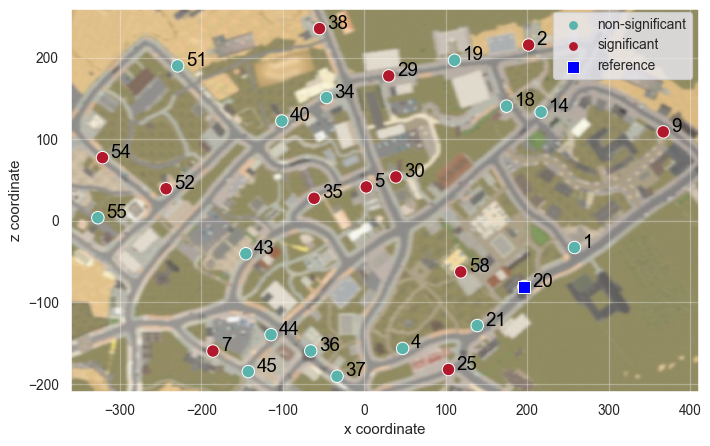
\includegraphics[width=150mm]{figures/significance_starting_locations_angular_error_map_23.png}
	\caption[Significance and meaningfulness (absolute angular deviation predicted by starting location)]{Significance and meaningfulness of LMM results of absolute angular deviation predicted by starting location}
	\label{fig:sig_angle_loc_map}
\end{figure}

In comparison to the starting location No. 20 (fast food restaurant) ,the reference point, the starting location No. 51 (wine shop) has the least difference in angular error degree to the reference and the starting location No. 9 (patisserie) the most. All three locations are meaningful locations.

\subsection{Reaction times}

The starting location No. 7 (bear) which is a non-meaningful location was chosen as the intercept for the model RT predicted by starting locations. This decision was made based on the comparison of medians of RT from each starting location to the overall median of 6.01s. Here the median was considered as the measure of central tendency because the medians were more normally distributed than means. The location No. 7 had median of 6.02s and the difference of 0.01s from the overall median. However, the starting location No. 29 (restaurant) had also the same difference from the overall median. Hence their mean difference to the overall mean of RT was also secondarily taken into account for the final choice. Location No. 7 had the smaller difference of 0.03s compared to the location No. 29 with the difference to mean of 0.55s. 

The LMM model was fitted using that reference location No. 7. The results (see table \ref{tab:RT_loc}) show a significant effect of 7 starting locations (listed in the table \ref{tab:sig_RT_loc}) on the dependent variable. From the 7 locations with a significant effect, 2 are meaningful locations and from the 20 non-significant locations, 12 are meaningful (see figure \ref{fig:sig_RT_loc_map}). The subject variance of the reaction times is 3.762.


\rowcolors{1}{light-gray}{light-gray}
\begin{longtable}{p{4cm}p{2cm}p{2cm}p{2cm}l}
	\hiderowcolors
	\caption[RT predicted by starting locations]{The results of the model RT predicted by starting locations} \\
	\hline \hline
	\multicolumn{1}{l}{Predictor} & \multicolumn{1}{l}{Coef. $\beta$} & \multicolumn{1}{l}{SE ($\beta$)} & \multicolumn{1}{l}{z-score} & \multicolumn{1}{r}{P$>|z|$} \\
	\hline \hline
	\showrowcolors
	Intercept       & 7.736  & 0.512 & 15.116 & 0.000 \\
	{[}Loc.1{]}     & -0.335 & 0.443 & -0.757 & 0.449 \\
	{[}Loc.2{]}     & -0.676 & 0.443 & -1.526 & 0.127 \\
	 \setrow{\bfseries} {[}Loc.4{]}     & \setrow{\bfseries}  -1.047 & \setrow{\bfseries}  0.443 & \setrow{\bfseries}  -2.365 & \setrow{\bfseries}  0.018  \\
	{[}Loc.5{]}     & 0.821  & 0.443 & 1.854  & 0.064 \\
	{[}Loc.9{]}     & -0.287 & 0.443 & -0.649 & 0.516 \\
	{[}Loc.14{]}    & 0.542  & 0.443 & 1.224  & 0.221 \\
	{[}Loc.18{]}    & 0.863  & 0.444 & 1.946  & 0.052 \\
	 \setrow{\bfseries} {[}Loc.19{]}    & \setrow{\bfseries}  -1.220 & \setrow{\bfseries}  0.443 & \setrow{\bfseries}  -2.755 & \setrow{\bfseries}  0.006  \\
	 \setrow{\bfseries} {[}Loc.20{]}    & \setrow{\bfseries}  -1.078 & \setrow{\bfseries}  0.443 & \setrow{\bfseries}  -2.435 & \setrow{\bfseries}  0.015 \\
	{[}Loc.21{]}    & -0.314 & 0.444 & -0.708 & 0.479 \\
	{[}Loc.25{]}    & -0.434 & 0.443 & -0.979 & 0.327 \\
	{[}Loc.29{]}    & -0.516 & 0.443 & -1.165 & 0.244 \\
	{[}Loc.30{]}    & 0.733  & 0.443 & 1.654  & 0.098 \\
	{[}Loc.34{]}    & 0.446  & 0.443 & 1.006  & 0.315 \\
	 \setrow{\bfseries} {[}Loc.35{]}    & \setrow{\bfseries}  1.323  & \setrow{\bfseries}  0.444 & \setrow{\bfseries}  2.978  & \setrow{\bfseries}  0.003   \\
	{[}Loc.36{]}    & -0.207 & 0.443 & -0.468 & 0.640   \\
	 \setrow{\bfseries} {[}Loc.37{]}    & \setrow{\bfseries}  0.945  & \setrow{\bfseries}  0.443 & \setrow{\bfseries}  2.134  & \setrow{\bfseries}  0.033   \\
	{[}Loc.38{]}    & -0.128 & 0.443 & -0.290 & 0.772 \\
	{[}Loc.40{]}    & 0.780  & 0.443 & 1.762  & 0.078 \\
	 \setrow{\bfseries} {[}Loc.43{]}    & \setrow{\bfseries}  0.929  & \setrow{\bfseries}  0.443 & \setrow{\bfseries}  2.098  & \setrow{\bfseries}  0.036   \\
	{[}Loc.44{]}    & -0.312 & 0.443 & -0.704 & 0.482 \\
	{[}Loc.45{]}    & 0.470  & 0.443 & 1.060  & 0.289 \\
	 \setrow{\bfseries} {[}Loc.51{]}    & \setrow{\bfseries} -1.042 & \setrow{\bfseries}  0.443 & \setrow{\bfseries}  -2.353 & \setrow{\bfseries}  0.019  \\
	{[}Loc.52{]}    & 0.340  & 0.444 & 0.766  & 0.444  \\
	{[}Loc.54{]}    & 0.438  & 0.444 & 0.987  & 0.323  \\
	{[}Loc.55{]}    & 0.128  & 0.443 & 0.289  & 0.772  \\
	{[}Loc.58{]}    & -0.290 & 0.443 & -0.655 & 0.512  \\
	subject\_id Var & 3.762  & 0.223 &  {}    &  {}    \\
	\hiderowcolors	\hline \hline
	\label{tab:RT_loc}
\end{longtable}

\rowcolors{1}{light-gray}{light-teal}
\begin{table}[h]
	\begin{center}
		\caption[Significant locations in RT predicted by starting location]{Significant locations in RT predicted by starting location}
		\vspace{10pt}
		\begin{tabular}{l l l r r} 
			\hiderowcolors
			\hline \hline
			{} & \setrow{\bfseries} Location ID-name & \setrow{\bfseries} mean & \setrow{\bfseries} median & \setrow{\bfseries} meaningfulness \\ [.7ex] 
			\hline\hline
			\showrowcolors
			1 & 4 (gorilla)		& 		6.69 &  	5.62	& non-meaningful	  \\ 
			\hline
			2 & 19 (bottle spray)		& 		6.52 & 5.28	 	& non-meaningful 	  \\
			3 & 20 (fast food) 			& 6.66 &	5.80	& meaningful  \\
			4 & 35 (underwater) 	& 	9.08 & 7.75		& non-meaningful	  \\
			5 & 37 (house) 		& 		8.68 & 6.69 		& non-meaningful  \\ 
			6 & 43 (daisy)		& 		8.66 	& 6.89	& non-meaningful  \\ 
			7 & 51 (wine shop)		& 		6.69 & 4.63 & meaningful  \\ 
			[1ex]
			\hline \hline
			\hiderowcolors
		\end{tabular}
		\label{tab:sig_RT_loc}
	\end{center}
\end{table}

\begin{figure}[!htb]
	\centering
	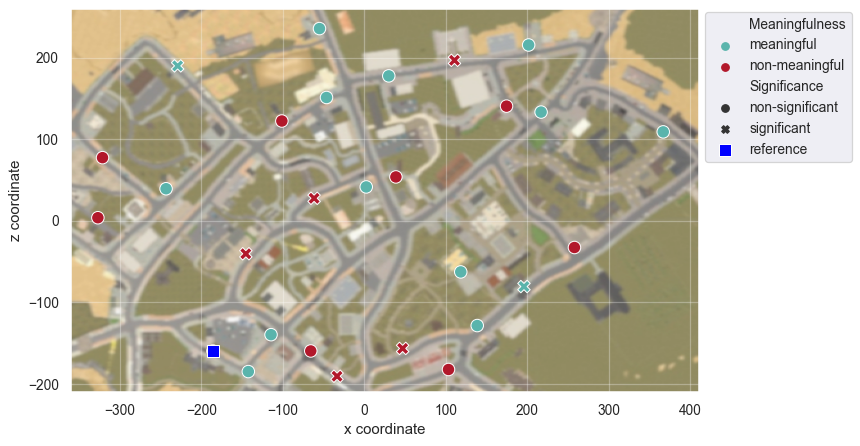
\includegraphics[width=150mm]{figures/significance_starting_locations_RT_map_23.png}
	\caption[Significance and meaningfulness (RT predicted by starting location)]{Significance and meaningfulness of LMM results of RT predicted by starting location}
	\label{fig:sig_RT_loc_map}
\end{figure}

In comparison to the starting location No. 7 (the reference point), the starting location No. 55 has the least difference in RT to the reference and the starting location No. 35 the most. All three locations are residential buildings.

%\section{Exploratory descriptive and analysis}
